\section{Construction (5 points)}

\begin{questions}
	\question[1] Construire un triangle $ABC$, tel que $AB$=\num{4.3} cm, $BC$ = \num{6.5} cm et $AC$=\num{8.3} cm.
	
	\question[1\half] Tracer la hauteur issue de $B$, son pied est le point $E$. Coder la figure.
	
	\question[1\half] Tracer la médiatrice de $[AC]$, elle coupe $(AC)$ en $D$ et $(BC)$ en F. Coder la figure
	
	\question[1] Tracer les segments $[BD]$ et $[EF]$. 
	\begin{solution}
		\begin{center}
			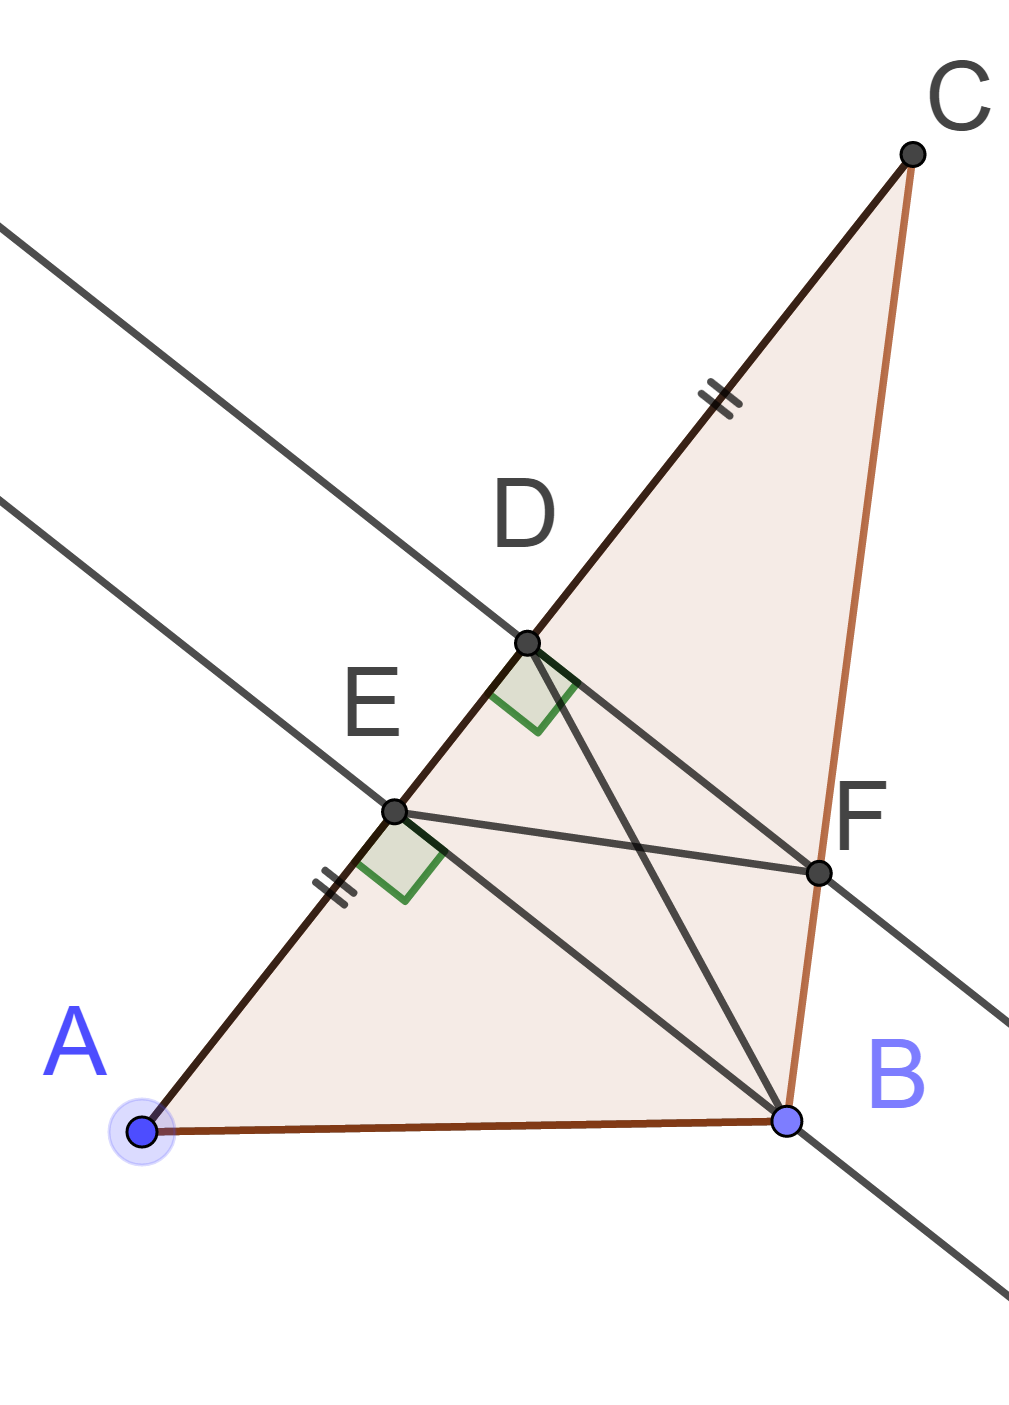
\includegraphics[scale=0.3]{img/ex2_fig}
		\end{center}
	\end{solution}
\end{questions}
  